\typeout{}\typeout{If latex fails to find aiaa-tc, read the README file!}

\documentclass[]{aiaa-tc}% insert '[draft]' option to show overfull boxes

 \title{Fisikoin: A Revolutionary Cryptocurrency for the Physical World}

 \author{
  Jacob Killelea%
    \thanks{Univ. Colorado at Boulder}
  \and Jesus Garnica%
    \thanks{Univ. California at San Francisco}\\
  \and
  Rebecca Schena%
    \thanks{Rhode Island School of Design}\\
 }

 % Define commands to assure consistent treatment throughout document
 \newcommand{\eqnref}[1]{(\ref{#1})}
 \newcommand{\class}[1]{\texttt{#1}}
 \newcommand{\package}[1]{\texttt{#1}}
 \newcommand{\file}[1]{\texttt{#1}}
 \newcommand{\BibTeX}{\textsc{Bib}\TeX}

\begin{document}

\maketitle

\begin{abstract}
We demonstrate a novel method for securiting a cryptocurrency using unhackable, 
untraceable methods. A combination of robust and flexible proof-of-work (POW) methods,
combined with rigid consensus structures are implemented in an entirely analog fasion 
that fosters community involvement and has minimual impact on the environment.
\end{abstract}

\section*{Nomenclature}

\begin{tabbing}
  XXX \= \kill% this line sets tab stop
  $J$ \> Jacobian Matrix \\
  $\beta$ \> Binder \\
  $f$ \> Residual value vector \\
  $x$ \> Variable value vector \\
  $F$ \> Force, N \\
  $m$ \> Mass, kg \\
  $c$ \> Coin \\
  $F$ \> Fisikoin \\
  $POW$ \> Proof of Work \\
  $\Delta x$ \> Variable displacement vector \\
  $\alpha$ \> Acceleration, m/s\textsuperscript{2} \\[5pt]
  \textit{Subscript}\\
  $i$ \> Variable number \\
 \end{tabbing}

\section{Introduction}


Lorem ipsum dolor sit amet, consectetur adipiscing elit. Proin porttitor eros at diam gravida, non tincidunt nibh imperdiet. Etiam gravida sed nibh eu tincidunt. Etiam malesuada, mi sed gravida consequat, ante ex commodo odio, non finibus lacus massa eu nisi. Cras eget ante ut dolor condimentum mollis. Sed mollis nisi lacus, ac pulvinar magna dapibus id. Maecenas ac euismod purus, non rhoncus nisi. Donec vulputate ante vitae eros tincidunt, vel aliquam ante egestas. Nullam tempor eros ut tristique fringilla. Proin vitae tortor at mauris efficitur scelerisque eget in risus. Vivamus est mi, semper eget diam eu, consequat pellentesque massa. In odio risus, tristique a mauris tristique, consectetur sollicitudin velit. Class aptent taciti sociosqu ad litora torquent per conubia nostra, per inceptos himenaeos. Pellentesque pulvinar sem non sem cursus ullamcorper.



\subsection{Background}

Morbi congue ac nisl id venenatis. Nullam augue ex, posuere molestie tincidunt sed, blandit faucibus ex. Nullam viverra lectus ut maximus semper. Donec venenatis libero dui, quis feugiat libero tincidunt et. Vivamus volutpat sit amet odio eu ornare. Ut cursus vehicula dui ac vulputate. Fusce massa turpis, placerat eu lectus sit amet, ultricies efficitur nunc. Pellentesque scelerisque porta ante ac dictum. Suspendisse ut nibh dapibus, porttitor velit id, tempus ipsum. Duis euismod dolor magna, sed rutrum tellus consectetur quis. Sed in ornare tortor. Nullam egestas ligula quis massa feugiat molestie. Nam ac eros non odio euismod eleifend. Lorem ipsum dolor sit amet, consectetur adipiscing elit. Donec nec dolor vel turpis ultricies semper id eget odio. Vestibulum dapibus odio ut urna commodo, egestas mollis urna blandit.


\subsubsection{Detail}

In hac habitasse platea dictumst. Nullam molestie nulla non finibus blandit. Pellentesque elementum viverra neque, nec faucibus diam tincidunt eget. Curabitur vel tempus dui. Aliquam euismod purus quis velit bibendum, ut aliquam velit cursus. Sed malesuada turpis vel bibendum dictum. Proin ipsum magna, posuere eu velit ac, dictum pulvinar lacus. Cras id laoreet odio. Nulla lectus ipsum, cursus nec tempor quis, eleifend at mauris. Vivamus pretium, quam vitae viverra efficitur, ex tellus porta magna, nec venenatis odio lacus in quam.


\section{Model}

Donec rhoncus, tellus id auctor euismod, augue velit dapibus risus, id gravida justo mi at quam. Pellentesque varius justo ac tellus lacinia cursus. Vivamus sed blandit dolor. Donec volutpat nisi tortor, sed mollis arcu efficitur eu. Etiam eu venenatis metus. Sed dui eros, volutpat vel venenatis id, laoreet sed ipsum. Sed nisl quam, bibendum eu viverra sed, lacinia vel enim. Mauris justo risus, ullamcorper a bibendum a, tristique eget justo. Morbi eget faucibus ligula, quis dignissim nibh. Etiam felis urna, tristique in purus ac, mattis posuere arcu. Morbi vitae mauris et arcu sagittis imperdiet. Vestibulum elementum enim ante, placerat suscipit leo viverra ut. Quisque eget justo commodo, venenatis turpis maximus, commodo ex. Nullam arcu eros, ullamcorper sed porta vel, hendrerit vitae risus.

Etiam ac nulla nec lectus commodo volutpat. Aliquam ullamcorper viverra urna vitae aliquet. Aliquam venenatis ullamcorper ante a faucibus. Nulla facilisi. Pellentesque at dignissim neque. Donec vestibulum ipsum ut odio dictum, sit amet luctus turpis laoreet. Donec efficitur velit vitae varius accumsan. Integer aliquam magna id tortor semper, sed pharetra eros dignissim. Vestibulum nec orci vel quam mattis suscipit. Donec ac ante diam. Vestibulum ipsum purus, placerat vitae convallis eu, pellentesque id ipsum.

We should probably include some math.
Here we begin with Eq.~(\ref{e:function}) that demonstrates some math
typesetting.
\begin{equation}
 \label{e:function}
 \int_{0}^{r_{2}} F(r,\varphi) \, dr \, d\varphi =
    \left[ \sigma r_{2}/(2\mu_{0}) \right] \cdot
    \int_{0}^{\infty} \exp(-\rho|z_{j}-z_{i}|) \, \lambda^{-1} 
\end{equation}
Eq.~(\ref{e:function}) is grand.
Some say it is due to Rebek.\cite{rebek:82bk}

\section{Results}

\begin{equation}
    log(log(log(log(\beta)))) = 999 \int_{me}^{you} POW \times j
\end{equation}

In this section we will introduce some figures and tables.
It can be seen in figure~\ref{f:magnetic_field} that magnetization is a
function of applied field.
\begin{figure}[htb]% order of placement preference: here, top, bottom
 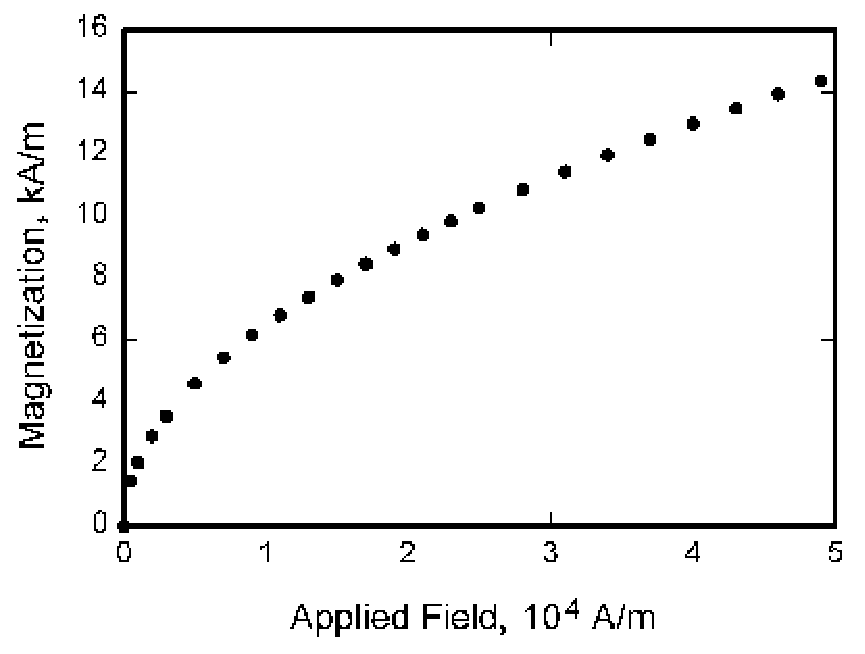
\includegraphics{figure_magnet}
 \caption{Magnetization as a function of applied field, which has
   borders so thick that they overwhelm the data and for some reason the
   ordinate label is rotated 90 degrees to make it difficult to
   read. This figure also demonstrates the dangers of using a bitmap
   as opposed to a vector image.}
 \label{f:magnetic_field}
\end{figure}
Sometimes writing meaningless text can be quiet easy, but other times
one is hard pressed to keep the words flowing.\footnote{And sometimes
things get carried away in endless detail.}
Meanwhile back in the other world, table~\ref{t:scheme_comparison} shows
a nifty comparison.
\begin{table}% no placement specified: defaults to here, top, bottom, page
 \begin{center}
  \caption{Variable and Fixed Coefficient Runge-Kutta Schemes as a
           Function of Reynolds Number}
  \label{t:scheme_comparison}
  \begin{tabular}{rrr}
       Re & Vary & Fixed \\\hline
        1 &  868 & 4,271 \\
       10 &  422 & 2,736 \\
       25 &  252 & 1,374 \\
       50 &  151 &   736 \\
      100 &  110 &   387 \\
      500 &   85 &   136 \\
    1,000 &   77 &   117 \\
    5,000 &   81 &    98 \\
   10,000 &   82 &    99
  \end{tabular}
 \end{center}
\end{table}

\section*{Appendix}

\begin{table}% no placement specified: defaults to here, top, bottom, page
    \begin{center}
        \caption{Original NESTLÉ TOLL HOUSE Chocolate Chip Cookies}
        \begin{tabular}{rr}
        \hline Prep Time & 15 Mins \\
        Cook Time & 9 Mins \\
        Cool Time & 15 Mins \\
        Yield & 5 dozen cookies \\
        \end{tabular}
    \end{center}
\end{table}

This famous classic American cookie is a treat no matter what the age or occasion.  
Enjoy it with a glass of cold milk.

\begin{enumerate}
\item Ingredients: 2 1/4 cups all-purpose flour 1 teaspoon baking soda 1 teaspoon salt 1 
    cup (2 sticks) butter, softened 3/4 cup granulated sugar 3/4 cup packed brown sugar 1 
    teaspoon vanilla extract 2 large eggs 2 cups (12-oz. pkg.) NESTLÉ® TOLL HOUSE® 
    Semi-Sweet Chocolate Morsels 1 cup chopped nuts 

\item PREHEAT oven to $375^\circ F$.

\item COMBINE flour, baking soda and salt in small bowl. Beat butter, granulated sugar, brown sugar and vanilla extract in large mixer bowl until creamy. Add eggs, one at a time, beating well after each addition. Gradually beat in flour mixture. Stir in morsels and nuts. Drop by rounded tablespoon onto ungreased baking sheets.

\item BAKE for 9 to 11 minutes or until golden brown. Cool on baking sheets for 2 minutes; remove to wire racks to cool completely.

\item PAN COOKIE VARIATION: Preheat oven to $350^\circ F$.  Grease 15 x 10-inch jelly-roll pan. Prepare dough as above. Spread into prepared pan. Bake for 20 to 25 minutes or 
until golden brown. Cool in pan on wire rack. Makes 4 dozen bars.
Step 5

* May be stored in refrigerator for up to 1 week or in freezer for up to 8 weeks.
Step 6

\item FOR HIGH ALTITUDE BAKING (5,200 feet):  Increase flour to 2 1/2 cups. Add 2 teaspoons water with flour and reduce both granulated sugar and brown sugar to 2/3 cup each. Bake drop cookies for 8 to 10 minutes and pan cookie for 17 to 19 minutes.

\end{enumerate}

\end{document}
